\section{Motivation}
There are many methods to create something new and they all begin with an idea that needs realization. The path to realization in some cases can involve simply building the final project; however, with Aerospace Engineering that is not the case. In order to achieve the end goal much planning is needed. A idea is formed, the feasibility is researched, it is designed, and then built. With many Aerospace projects, designing a cutting edge project requires accurate physical modeling in order confirm the feasibility of the design and examine the effects of iterations. Therefore, the field of Aerospace simulation and modeling is a large and extensive field. It is one which is constantly changing and expanding as computing power becomes exponentially stronger. The boom in computing power has opened the door to this thesis. \par

\begin{figure}[h]
    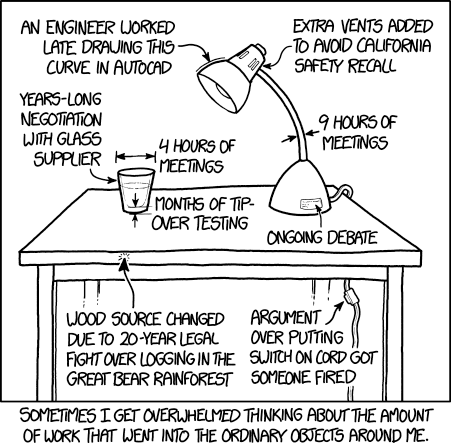
\includegraphics[width=.5\textwidth]{figures/work.png}
    \centering
    \caption{Example of various engineering design tasks \cite{xkcd}}
    \label{fig:xkcd}
\end{figure}

\indent Computational Fluid Dynamics (CFD) is the field of study which deals with creating simulations of fluids. This is a critical part of Aerospace design and analysis. Viscous fluid dynamics are completely described through the Navier-Stokes Equations.

\Needspace{12\baselineskip}
\begin{equation}
    \label{eqn:navier_1}
    \partial u_i + R u_j \partial u_i = -\partial \rho + \nabla u_i + E_i 
\end{equation}
\begin{equation}
    \label{eqn:navier_2}
        \partial_j u_j = 0  
\end{equation}
\(u_i\) = Velocity components (m/s) \newline
\(\rho\) = Pressure (Pa) \newline
\(E_i\) = External Forces (N) \newline
\(R\) = Reynolds number \(R = U d / \upnu \)  \par

\indent The Navier-Stokes equations, seen in  \ref{eqn:navier_1} and \ref{eqn:navier_2}\cite{navier_eqns}, are unfortunately impossible to solve analytically for the majority of fluid cases. They must be solved numerically, whose accuracy increases ask computational power increases. CFD capability and power has been steadily increasing along with computer power. CFD is currently an accepted and reliable industry tool for analysis across many disciplines. However, computers continue to get stronger which allows for more complicated techniques to be used for more unique scenarios. \par

\indent A large part of Aerospace research involves states of matter where the particles are very spread out. Atmospheric reentry of spacecraft, objects in Low Earth Orbit, planes flying at extremely high altitudes, and interactions with plasma all interact with fluids whose particles are relatively far apart from each other. This relative spacing can be measured through the knudsen number, seen in Equation \ref{eqn:knudsen}. \par

\Needspace{7\baselineskip}
\begin{equation}
    \label{eqn:knudsen}
    Kn = \frac{\lambda}{L}
\end{equation}
\(Kn\) = Knudsen number (non-dimensional) \newline
\(\lambda\) = Mean free path (m) \newline
\(L\) = Characteristic length (m) \par


\begin{figure}
    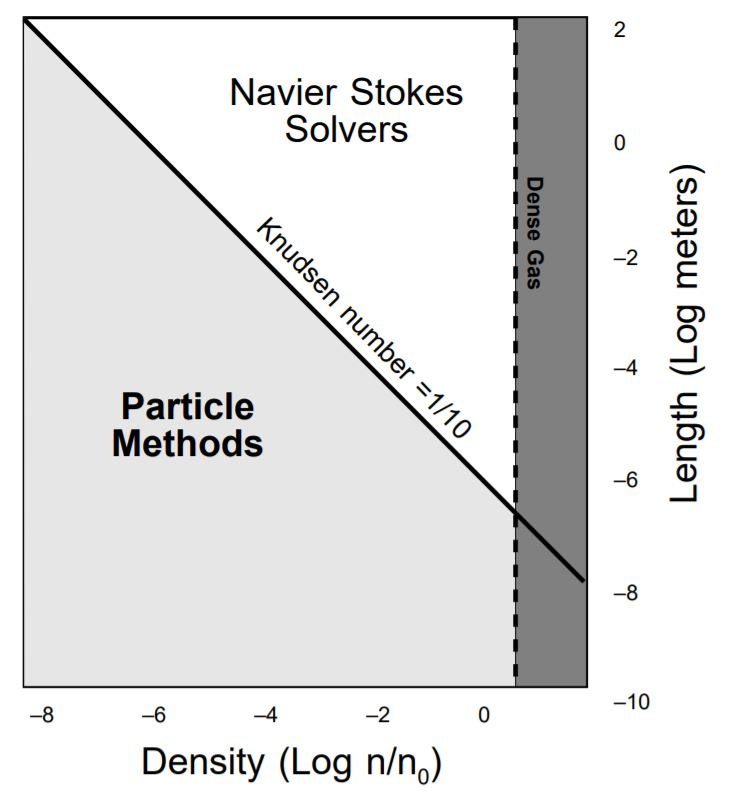
\includegraphics[width=.55\textwidth]{figures/navier.JPG}
    \centering
    \caption{Appropriate Simulation Models by Knudsen number \newline \cite{navier} }
    \label{fig:navier}
\end{figure}


\indent The mean free path is a measure of how far particles move before interacting with other particles and the characteristic length is a description of the basic length scale of the problem at hand. The ratio of the two (the knudsen number) shows their relative differences and, therefore, measures whether continuum is a good assumption for that fluid. When the knudsen number is very low ( \(\sim10^{-3}\) ) the particles collide much more often than they move the characteristic length, which means that a continuum assumption is valid. However, as seen in Figure \ref{fig:navier}, when the knudsen number is large ( \(\sim10^{1}\) and up ) the continuum assumption, and by inference the Navier-Stokes equations, are no longer valid. \par 

\indent There is another set of equations which can solve high knudsen number problems. This is the Boltzmann equation, shown in kinematic form for elastic interaction of particles in a plasma by Equation \ref{eqn:boltzmann} \cite{boltzmann}. It is based upon the statistical distribution of particles and their momentum. \par

\Needspace{3\baselineskip}
\begin{equation}
    \label{eqn:boltzmann}
    \frac{\partial f_i}{\partial t} + \vec{v_i} \cdot \frac{\partial f_i}{\partial \vec{r}} + \vec{F_i} \cdot \frac{\partial f_i}{\partial \vec{v_i}} = \sum_j \int_0^\infty \int_0^{2\pi} \int_0^\infty  [ f_i(v_i^\prime) f_j (v_j^\prime) - f_i (v_i) f_j (v_j) ] g_{ij} b \text{d} b \text{d} \epsilon \text{d} v_j
\end{equation}
\(F\) = Force acting on the particle \newline
\(g_{ij}\) = Initial relative velocity between particles \newline
\(b\) = impact parameter \newline
\(\epsilon\) = Azimuth angle \newline
\(\prime\) = Functions for post-collision \newline
\(f(v)\) = Particle distribution function \newline
\(i \: \text{and} \: j\) =  \(i\)th and \(j\)th species \newline
\(v\)   = Velocity  \par

\indent The Boltzmann equation can be solved for a few select unique cases. However, like the Navier-Stokes equations it must be solved numerically. To solve the equation itself numerically is a large task, considering the triple integral and the unknown way to find an accurate function for the particle distribution. It would follow that a discretion of the Boltzmann equation would be helpful. This is where a particle based code begins to make sense. \par

\indent The most basic algorithm for a particle based simulation is to keep track of every particle in the domain and calculate every collision with other particles and walls depending on the particles relative distances. While this algorithm, called Molecular Dynamics (MD), is a valid algorithm, computers are not strong enough currently to create meaningfully results from such a computationally heavy solution. This is where Direct Simulation Monte Carlo (DSMC) comes into play. DSMC was introduced in 1963\cite{dsmc_speed}, one year before the computer language BASIC was created\cite{basic}. Back then, it was seen as an inferior method to continuum solutions on account of the larger processing power required and that it seemed to abandon concrete mathematical solutions \cite{dsmc_speed}. Eventually it was shown that the limit as timestep and grid size approached 0 of a DSMC simulation was a solution to the Boltzmann equation\cite{bird_dsmc}. Through the years DSMC has gained respect and now is well known in the fluid modeling community as a standard for high knudsen number flow simulation methods.\par

\begin{quote}
    "The Direct Simulation Monte Carlo, or DSMC, method proved a probabilistic physical simulation of a gas flow by simultaneously following the motion of representative model molecules in a physical space." \cite{bird_dsmc}
\end{quote}


\begin{figure}
    \centering
  \begin{minipage}[b]{0.49\textwidth}
    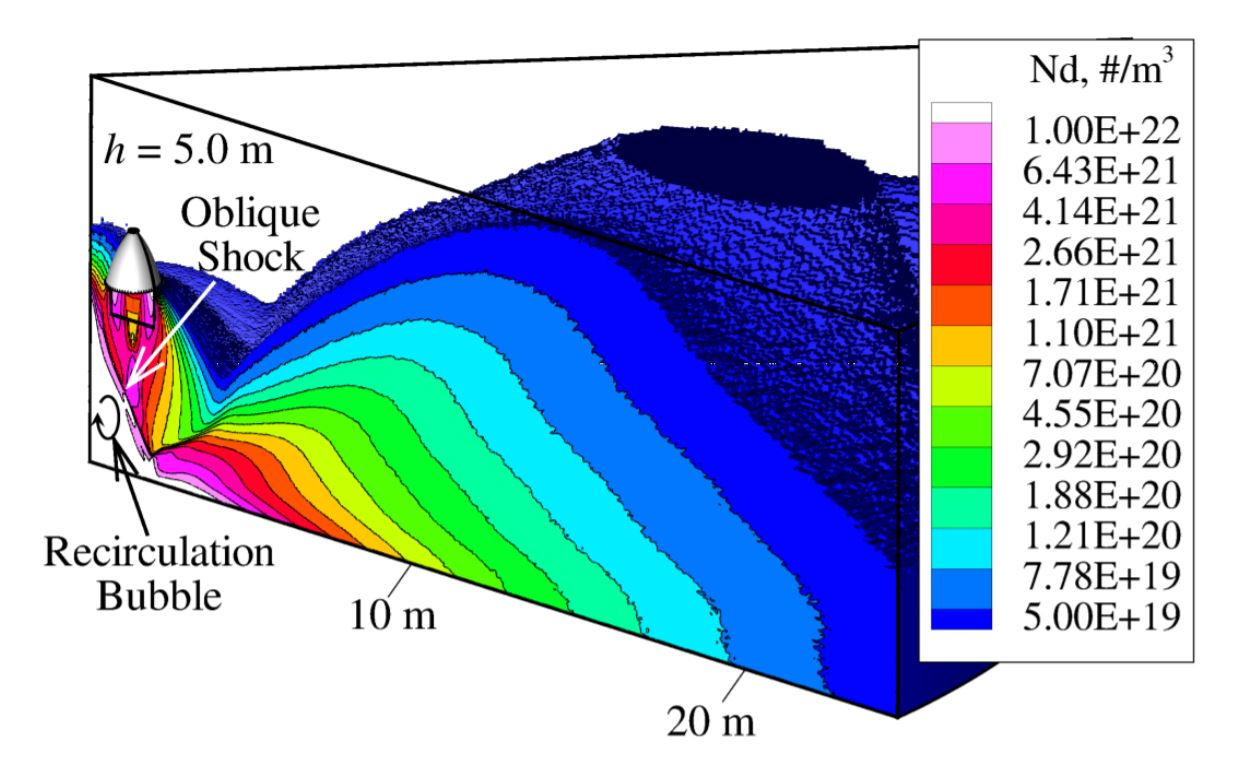
\includegraphics[width=\textwidth]{figures/hover_rocket.JPG}
  \end{minipage} %
  \begin{minipage}[b]{0.49\textwidth}
    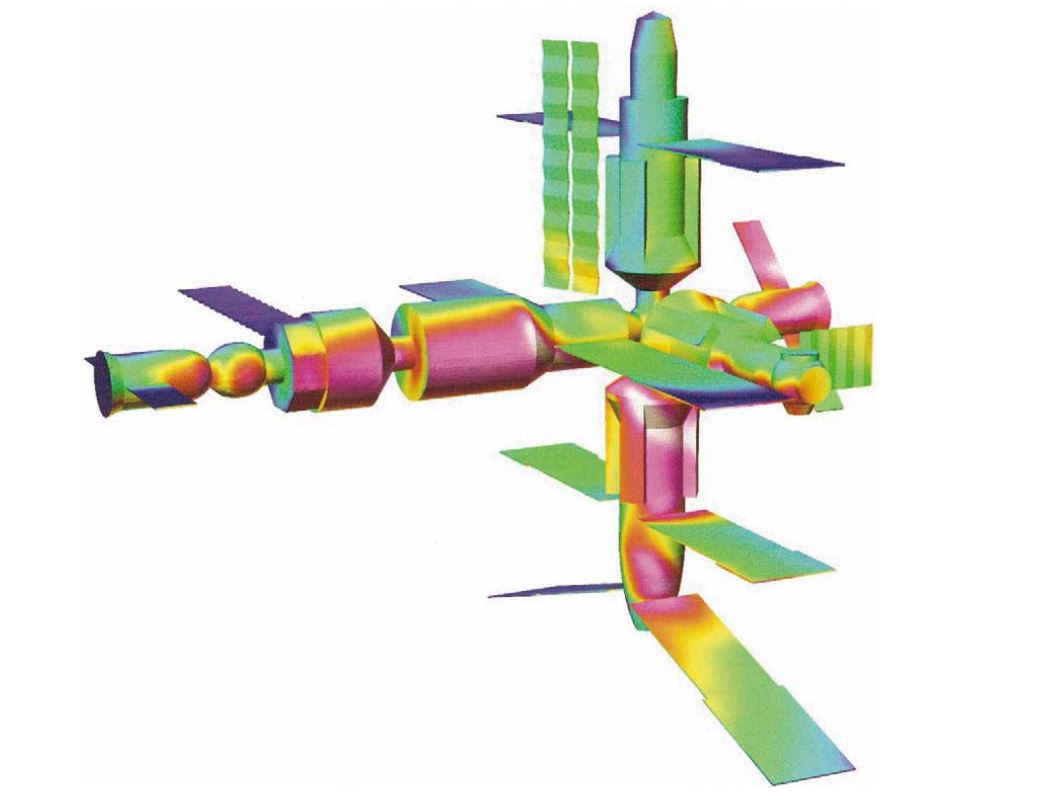
\includegraphics[width=\textwidth]{figures/mir_shuttle.JPG}

  \end{minipage}
  \caption[DSMC Application Examples]{DSMC Application Examples (top) A rocket lander hovering 5 m above the surface \cite{hover_rocket}. (bottom) Predicted surface pressure on Mir from the Space Shuttle RCS during docking \cite{mir_shuttle}.}
  \label{fig:dsmc_application}
\end{figure}

\indent DSMC fits into an important gap in fluid simulation methods. It is a particle based method, which allows it to accurately model high knudsen number simulations in which continuum codes break down. But it is also is based on probability and statistics and therefore allows critical computation time saving mathematics and algorithms to allow DSMC to be on par with legacy continuum methods. It simulates many super-particles in a domain, each of which is comprised of millions of physical particles, and uses probability and statistics to determine collisions surface interactions. This allows for a larger amount of high knudsen number scenarios to be simulated, including important astronautics applications. As seen in Figure \ref{fig:dsmc_application}, DSMC is now used for many important Aerospace analysis tasks. \par


\indent Unfortunately, DSMC alone does not account for a large area of aerospace research, plasma. Plasma exists when there are a large amount of ions and enough high energy electrons to keep ionizing the gas. As seen in Table \ref{tab:plasma}, plasma can exist in many various situations and environments. Even common place things like lightning and a candle flame contain plasma. There are two large areas of aerospace research which take place within a plasma environment: Atmospheric Re-entry and Electric Propulsion. Both exist in a high knudsen number environment, but include charged particles. Therefore, DSMC is not enough to model these situations. \par


\begin{table}
\label{tab:plasma}
\caption{Various Plasmas\cite{plasma_table}}
\vspace{0.3cm}
\begin{center}
\begin{tabular}{|lll|}
\hline
Plasma Type          & n (cm\textsuperscript{-3}) & T (eV)                  \\ \hline
Interstellar gas     & 1                        & 1                     \\
Solar Corona         & 10\textsuperscript{3}    & 1                     \\
Hot Plasma           & 10\textsuperscript{14}   & 10\textsuperscript{2} \\
Thermonuclear Plasma & 10\textsuperscript{15}   & 10\textsuperscript{4} \\
Laser Plasma         & 10\textsuperscript{20}   & 10\textsuperscript{2} \\ \hline
\end{tabular}
\end{center}
\end{table}

\indent Plasma is comprised of, on average, equal parts of negative electrons and positive ions, otherwise known as quasi-neutrality. However, there can be systematic (electric thruster) or random (solar wind) fluctuations which cause a local net charge. This fact means that the plasma will create electric forces which in turn effect the particles in a plasma. This is why DSMC cannot simulate charged particles, it only moves and collides the particles, it does not have a mechanism to calculate the electric force and update the particles velocities. This is where the Particle In Cell (PIC) method comes in. \par

\indent The PIC method is a standard method to calculate the force on electrically charged particles in a particle type model. It is based on a mesh system comprised of nodes, upon which field calculations are made. The mathematics of charged particles forces in terms of PIC will be discusses in Chapter \ref{chap:charge}. PIC however, does not account for collisions between particles. To accuratly model a plasma for aerospace research, collisions between particles should be accounted for. This naturally leads to the necessity for a DSMC-PIC combined method. The same mesh can be used for calculating collisions and macro-properties through the DSMC side as well as being used to calculate the fields in the domain and how they affect the particle's velocities. This allows for a program which can simulate a large number of various scenarious. \par


\indent One scenario within Aerospace research for which a DSMC-PIC simulation is optimal is electric propulsion. There are three main methods of spacecraft propulsion: cold gas, chemical, and electric. Chemical is the classic big fire and smoke engines used to put spacecraft and humans into orbit. Cold gas is simply expelling pressurized gas to provide thrust. Electric propulsion uses electricity to create a higher thrust and more efficient engines on spacecraft. Electric propulsion can either be electrostatic, electrothermal, or electromagnetic, however a nearly universal commonality in electric thrusters is that the expellled gas, in the form of a plume, is usually in a plasma state. An electric propulsion engine, in this case an ion engine, is seen in Figure \ref{fig:ion_thruster}. This figure shows the neutral propelant gas being ionize din the chamber, then the ions are accelerated out through magnetic grids to create thrust. This results in a plasma plume. Being that the spacecraft is in space and that the thrusters do not expel dense amounts of gas, this plasma fits right into the realm of a DSMC-PIC simulation. In this lies the motivation for this thesis. \par


\begin{figure}
    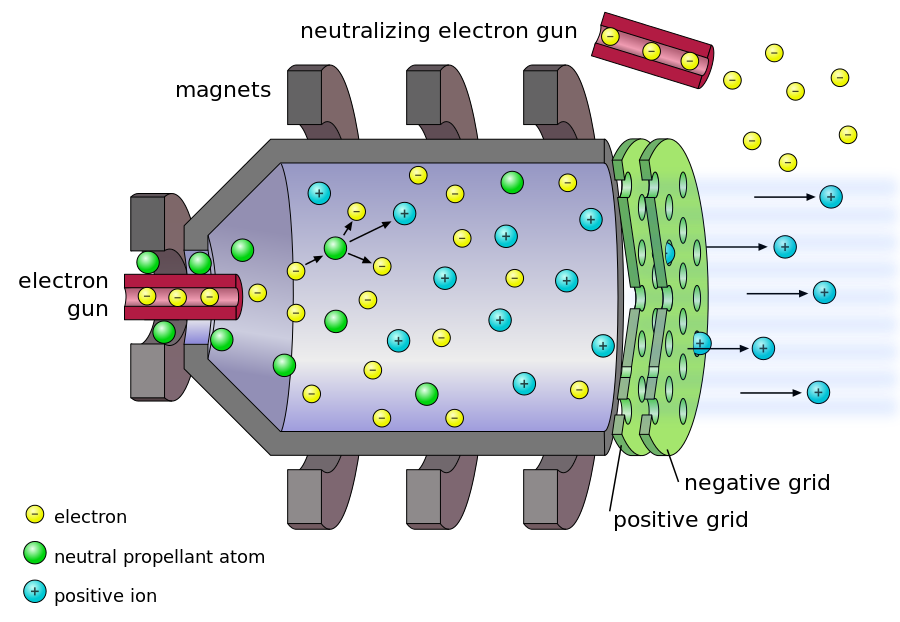
\includegraphics[width=.85\textwidth]{figures/ion_thruster.png}
    \centering
    \caption{Diagram of an Ion Thruster \cite{ion_thruster} }
    \label{fig:ion_thruster}
\end{figure}

%\footnote{By Oona Räisänen - Own work; self made in Inkscape. Based on File:Ion_engine.gif., CC BY-SA 3.0, https://commons.wikimedia.org/w/index.php?curid=20308289}



\section{Overarching Goal}
This thesis is one project in a series of projects. The end goal is to have a Cal Poly homegrown simulation that can simulate an entire electric thruster. This is a task that has not yet been accomplished in manner accessible to university researchers cite{}. A simulation of a full electric thruster requires a fluid based simulation for the gas inside the thruster and then a rarefied gas code for the exhaust plume. There are not codes that have been built as one simulation, instead researcher attempt to join a fluid code and rarefied gas code together. Cal Poly’s Aerospace department is unique in that a fluid code and a rarefied gas code are being developed from the ground up in the exact same manner. The early developers and advisors worked together to build these codes to be compatible from the beginning. \par

\indent This thesis is the third project of the homegrown DSMC code, code name SINATRA, which will be able to simulate the thruster’s plasma exhaust plume. The first three developers worked together in a staggered capacity to build SINATRA up to a working DSMC-PIC code. The first, David Galvez, developed the base framework and kinematics \cite{Galvez2018a}. Next Robert Alliston built up the collisions and particle models cite{Mac’s Thesis}. This thesis adds charged particle simulation to SINATRA. At the same time as this thesis, Anthony Gay is building the fluid side simulation. Intentionally many things will be common between the codes. They are both written in C++ and are class based. They share the same process control items including the execution style, distribution method, and the other systems engineering items shown in Chapter \ref{chap:systems}. They share the same mesh type, input class, and other items to help them work together as one simulation. A future project is slated that will take both simulations and build the interaction system to connect them across each timestep.
. 
